%%%%%%%%%%%%%%%%%%%%%%%%%%%%%%%%%%%%%%%%%%%%%%%%%%%%%%%%%%%%%%%%%%%
%%% Documento LaTeX 																						%%%
%%%%%%%%%%%%%%%%%%%%%%%%%%%%%%%%%%%%%%%%%%%%%%%%%%%%%%%%%%%%%%%%%%%
% Título:		Capítulo 3
% Autor:  	Ignacio Moreno Doblas
% Fecha:  	2014-02-01
% Versión:	0.5.0
%%%%%%%%%%%%%%%%%%%%%%%%%%%%%%%%%%%%%%%%%%%%%%%%%%%%%%%%%%%%%%%%%%%
\chapterbegin{Plan de pruebas y verificación}
\label{chp:App}
%\minitoc
\section{Funcionamiento de la aplicación}
\begin{figure}[h] \centering
 \begin{minipage}{0.45\textwidth}\centering
    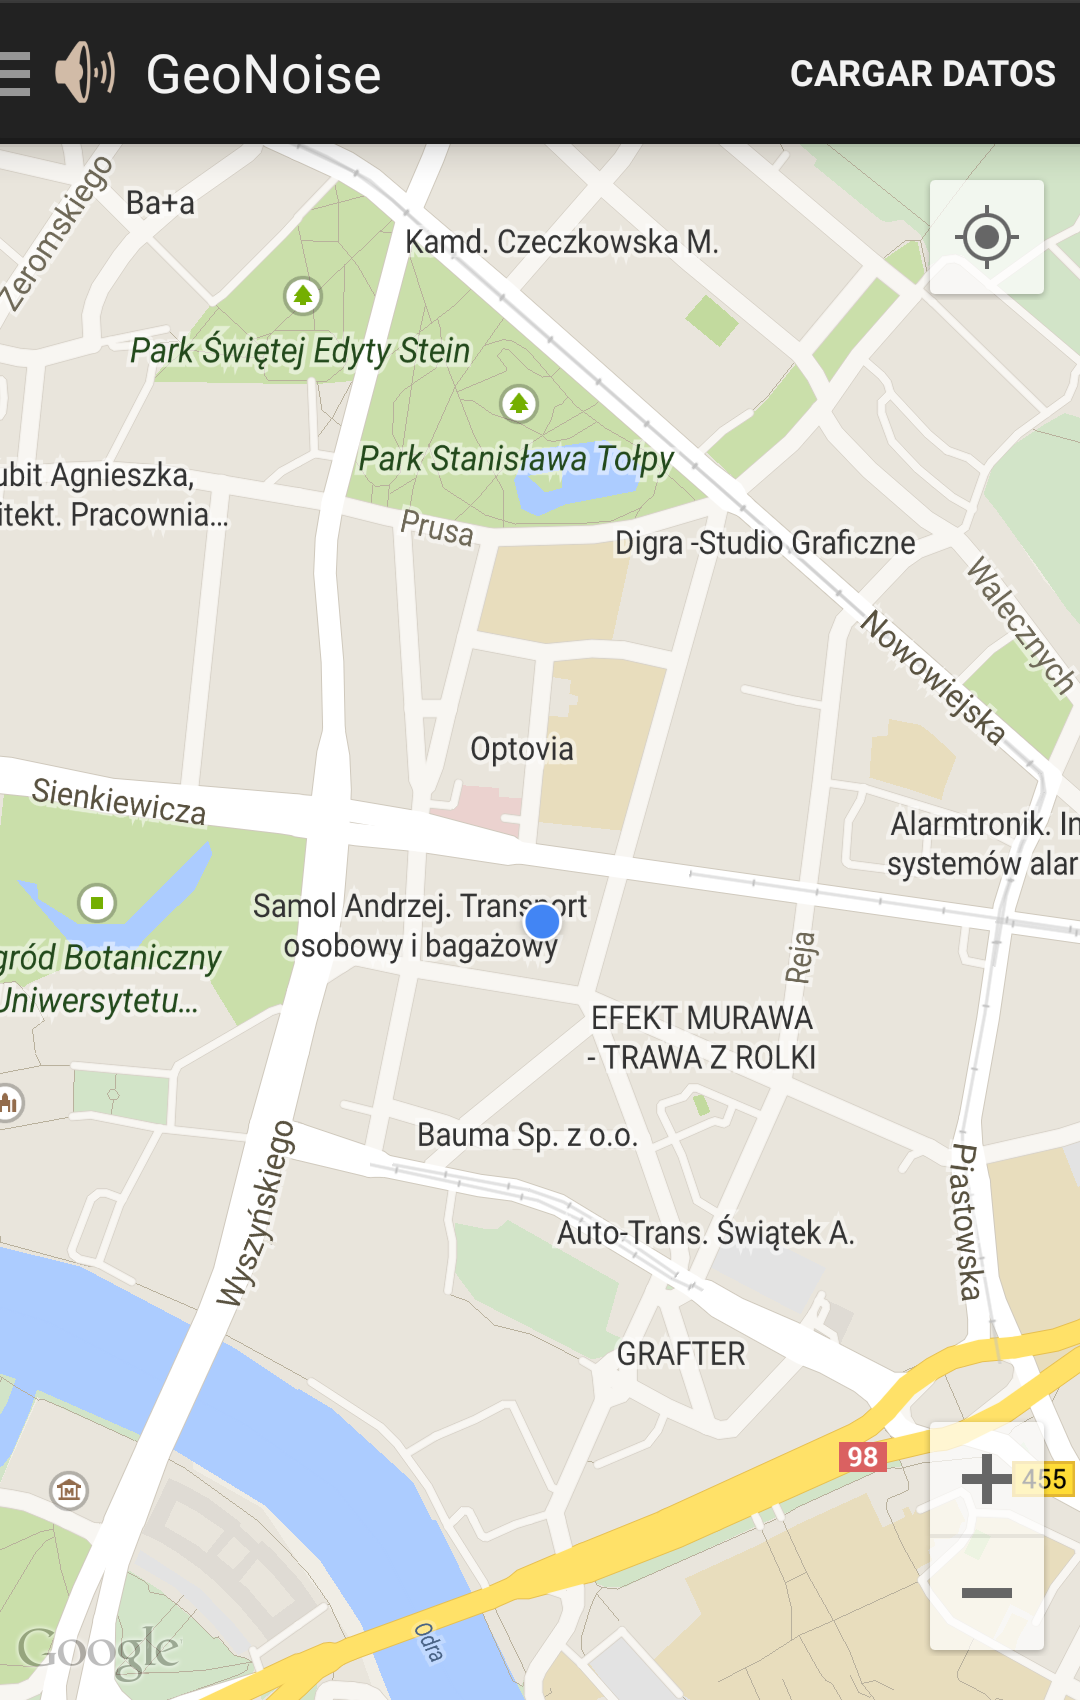
\includegraphics[height=11cm]{graphs/screen_location.png} \caption{Fragmento \ttw{Mapa de Calor}. }\label{fig:screen:location}
\end{minipage}
\hfill
 \begin{minipage}{0.45\textwidth}\centering
    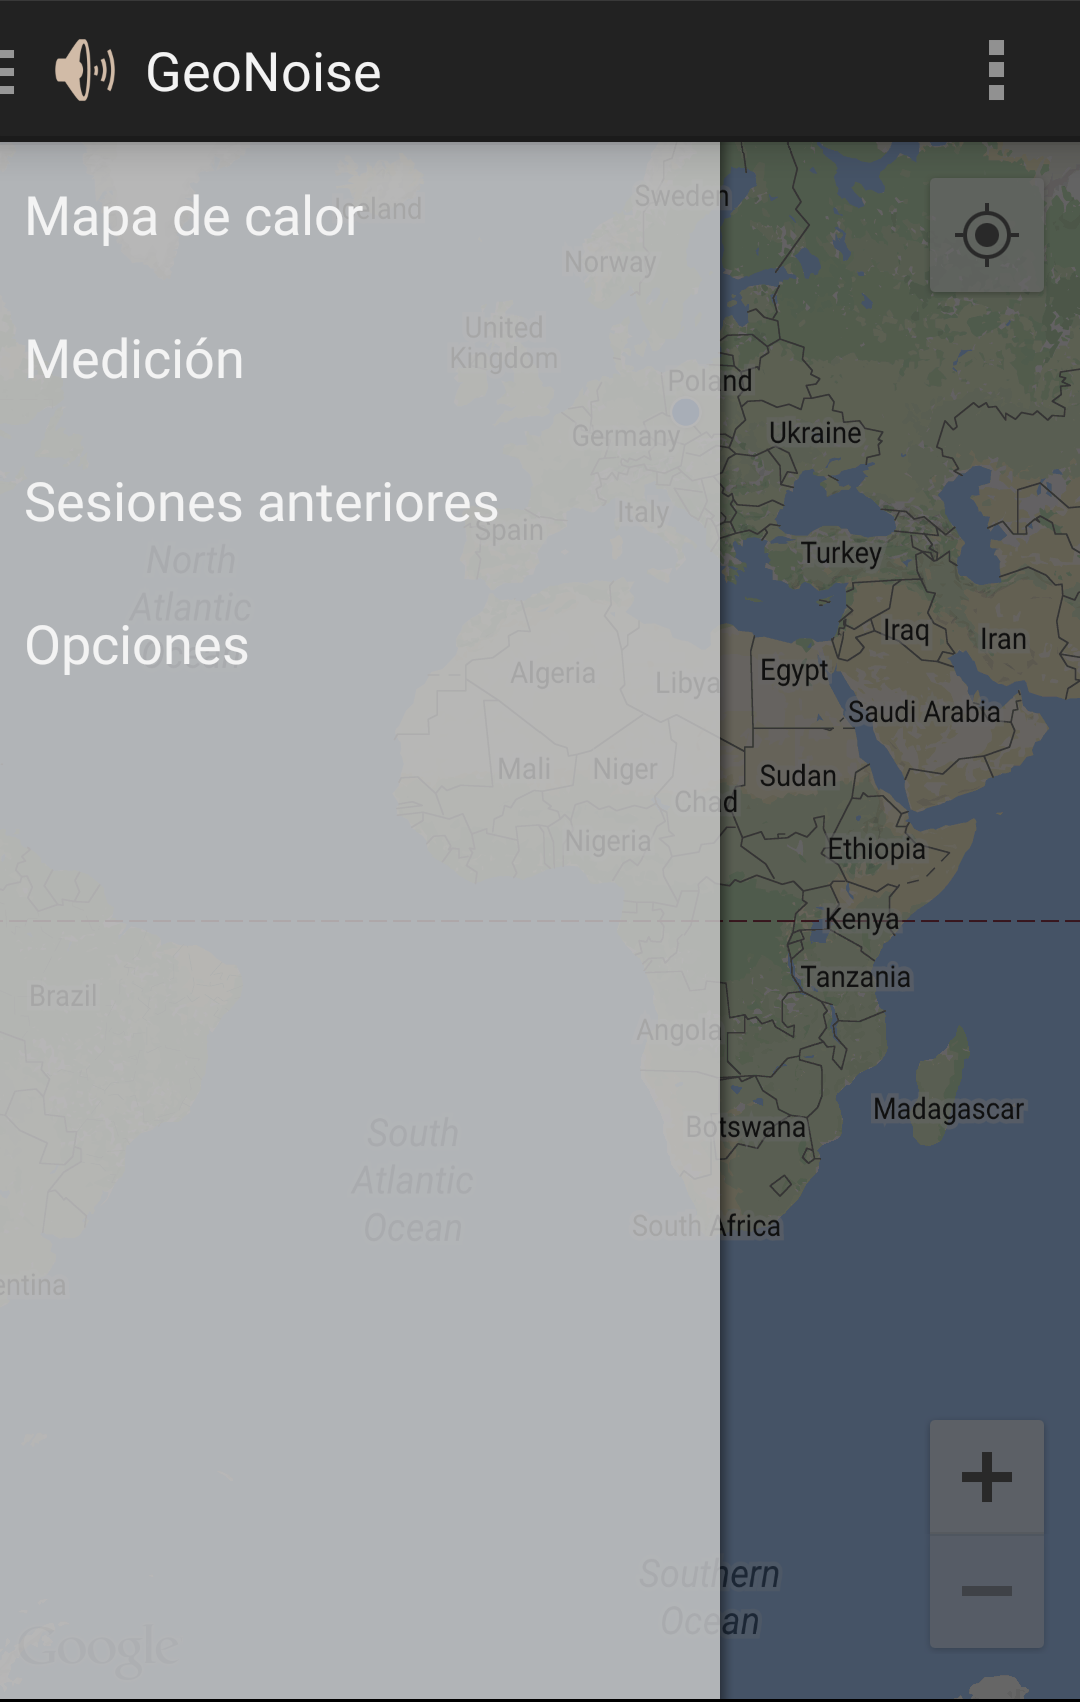
\includegraphics[height=11cm]{graphs/navdrawer.png} \caption{Cajón de navegación abierto.}\label{fig:screen:navdrawer}
\end{minipage}
\end{figure}

\begin{figure}[h] \centering
 \begin{minipage}{0.45\textwidth}\centering
    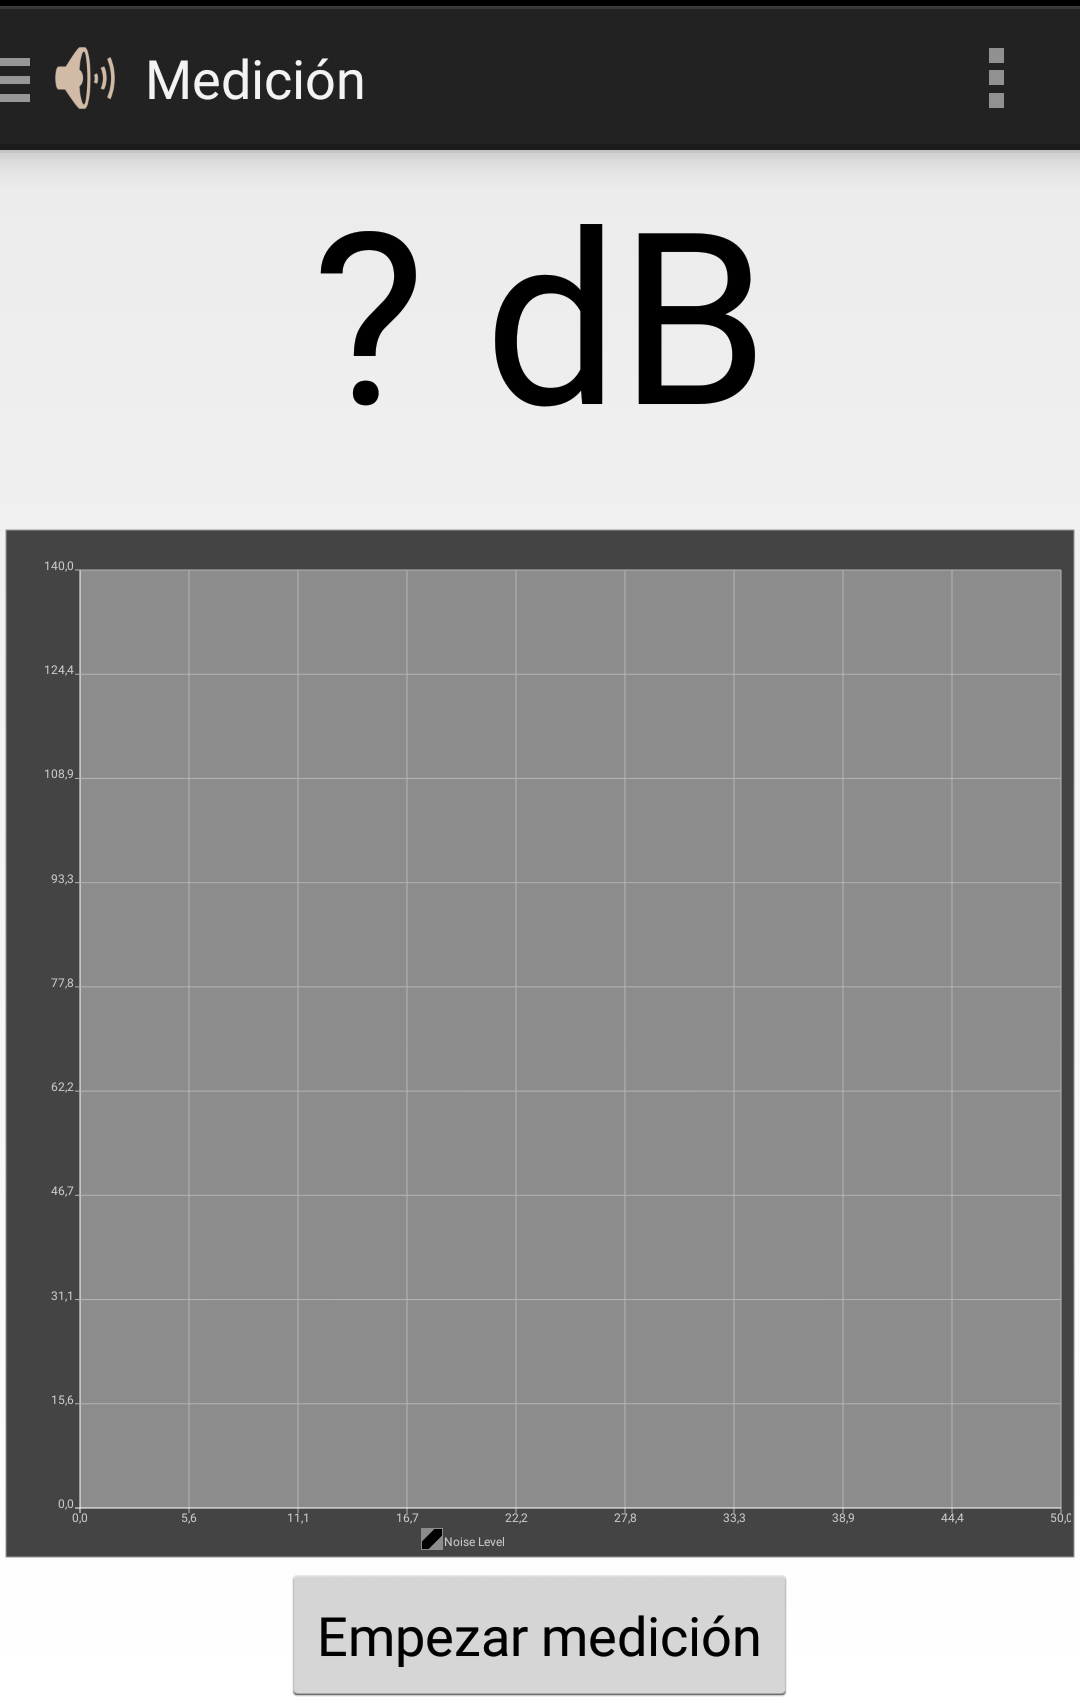
\includegraphics[height=11cm]{graphs/measure-empty.png} \caption{Fragmento \ttw{Medición} en reposo.}\label{fig:screen:measure-empty}
 \end{minipage}
 \hfill
\begin{minipage}{0.45\textwidth}\centering
    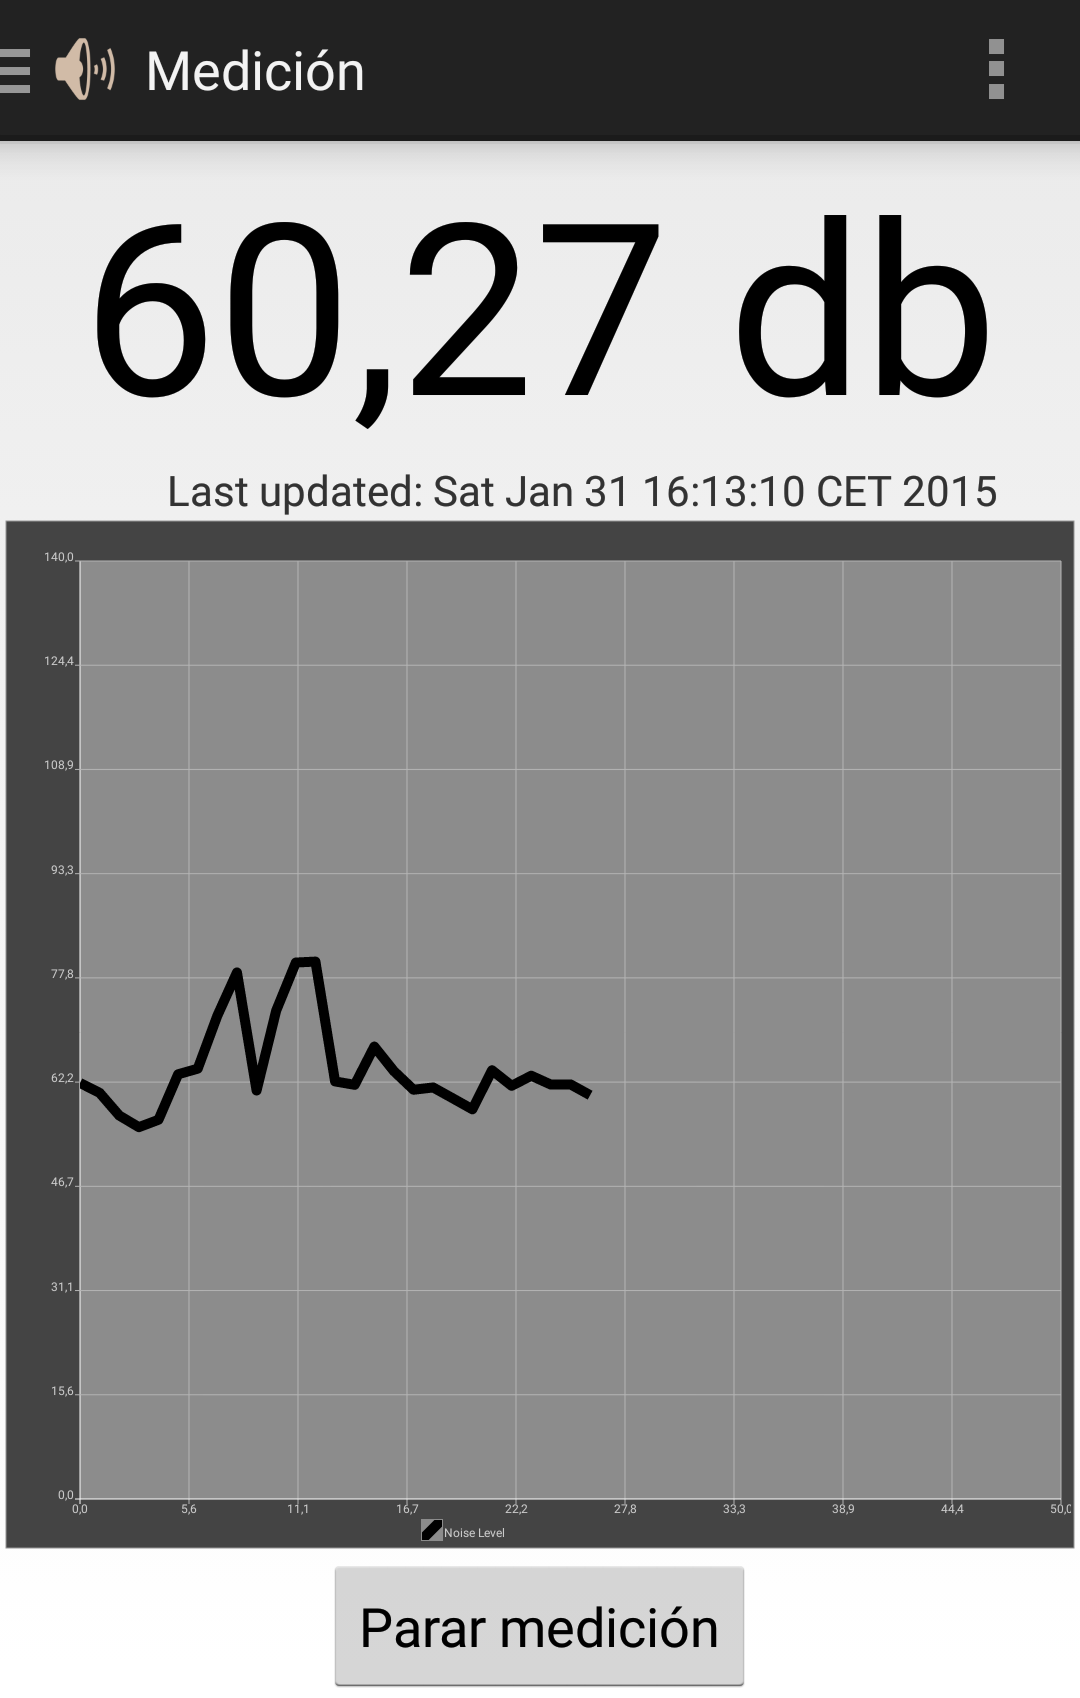
\includegraphics[height=11cm]{graphs/screen_measure.png} \caption{Fragmento \ttw{Medición} durante una medición.}\label{fig:screen:measure}
\end{minipage}
\end{figure}

\begin{figure}[h] \centering%
 \begin{minipage}{0.45\textwidth}\centering%
    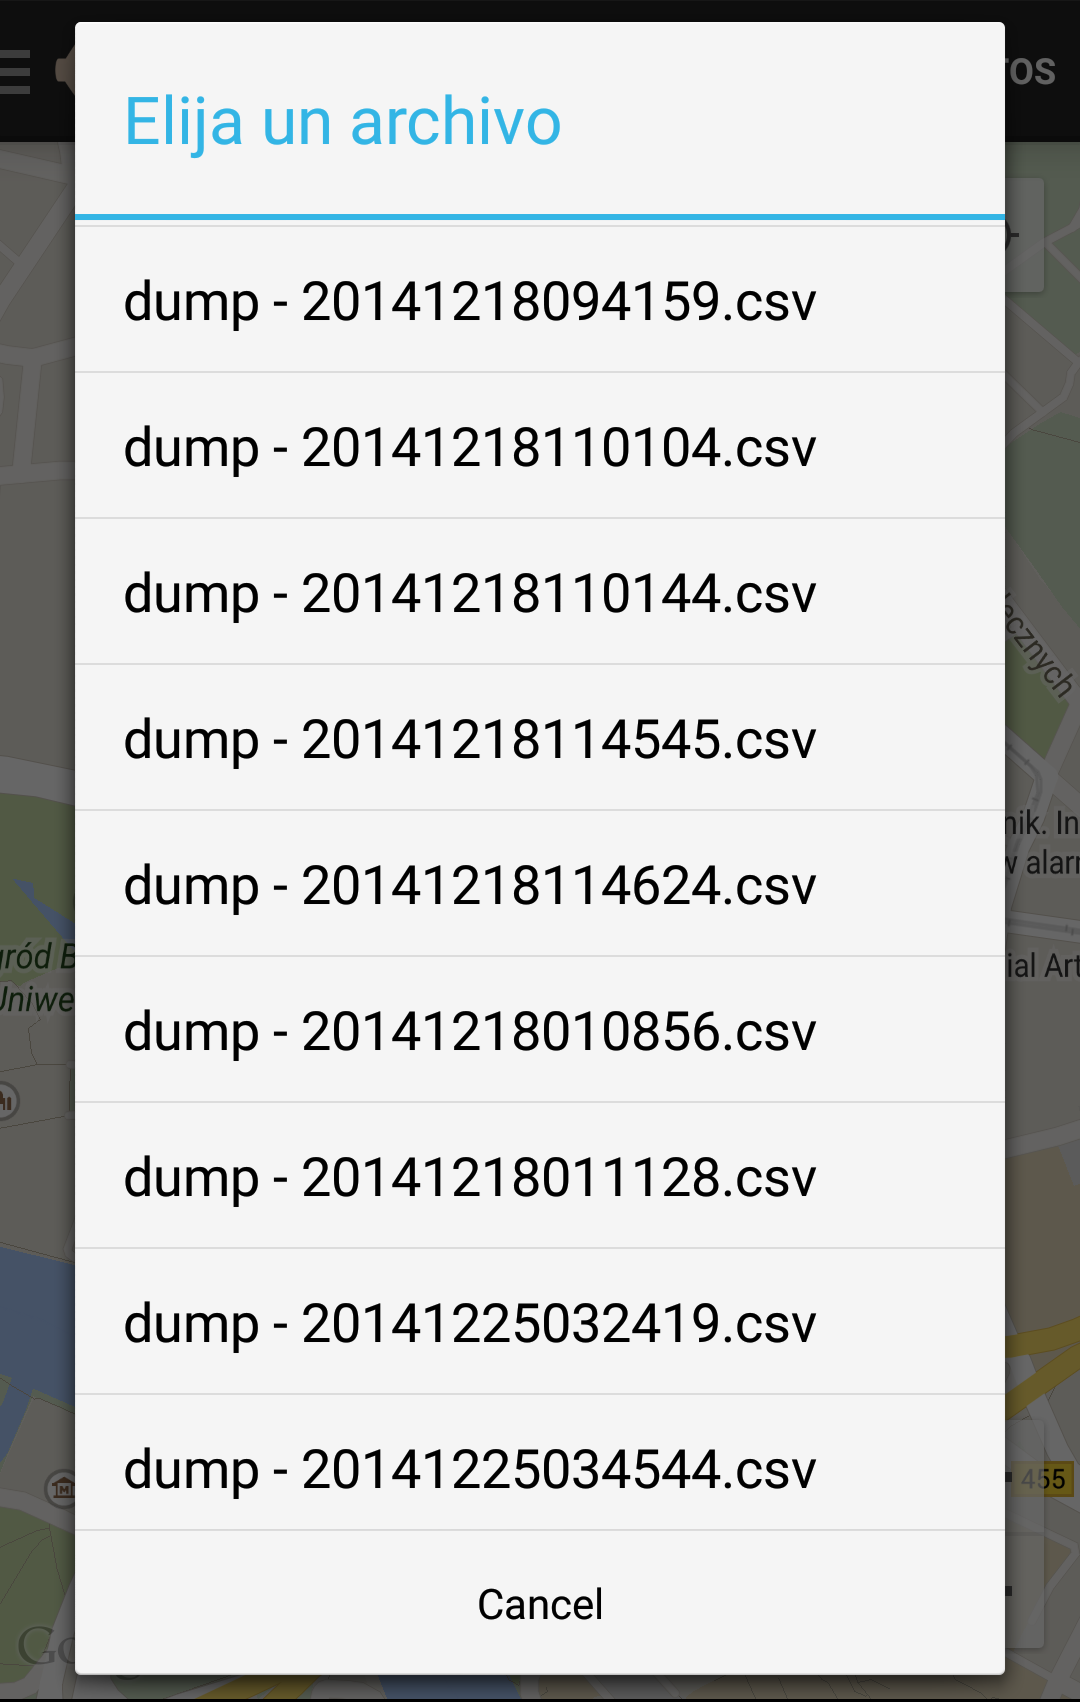
\includegraphics[height=11cm]{graphs/filepicker.png} \caption{Diálogo para la elección del archivo de sesión.}\label{fig:screen:filepicker}%
 \end{minipage}
 \hfill
\begin{minipage}{0.45\textwidth}\centering%
 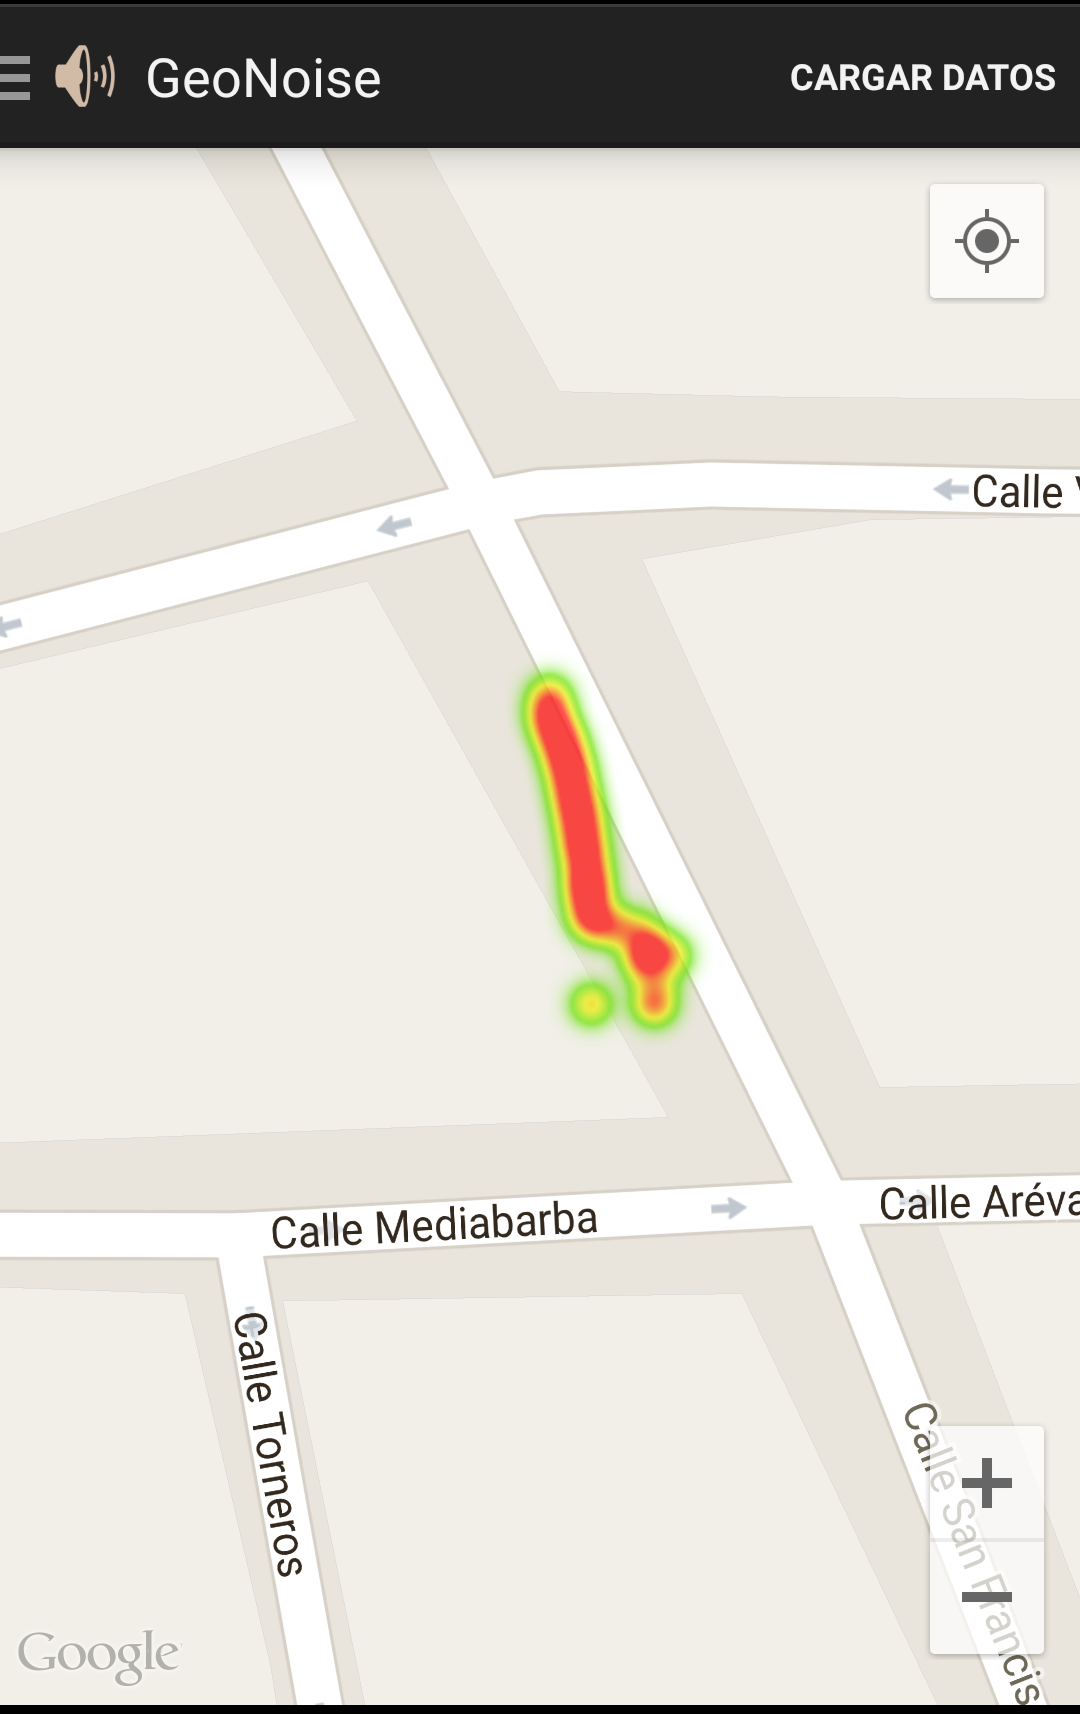
\includegraphics[height=11cm]{graphs/screen_heatmap.png} \caption{Fragmento \ttw{Mapa de Calor} mostrando datos cargados.}\label{fig:screen:heatmap}
\end{minipage}
\end{figure}

\begin{figure}[h] \centering%
 \begin{minipage}{0.45\textwidth}\centering%
    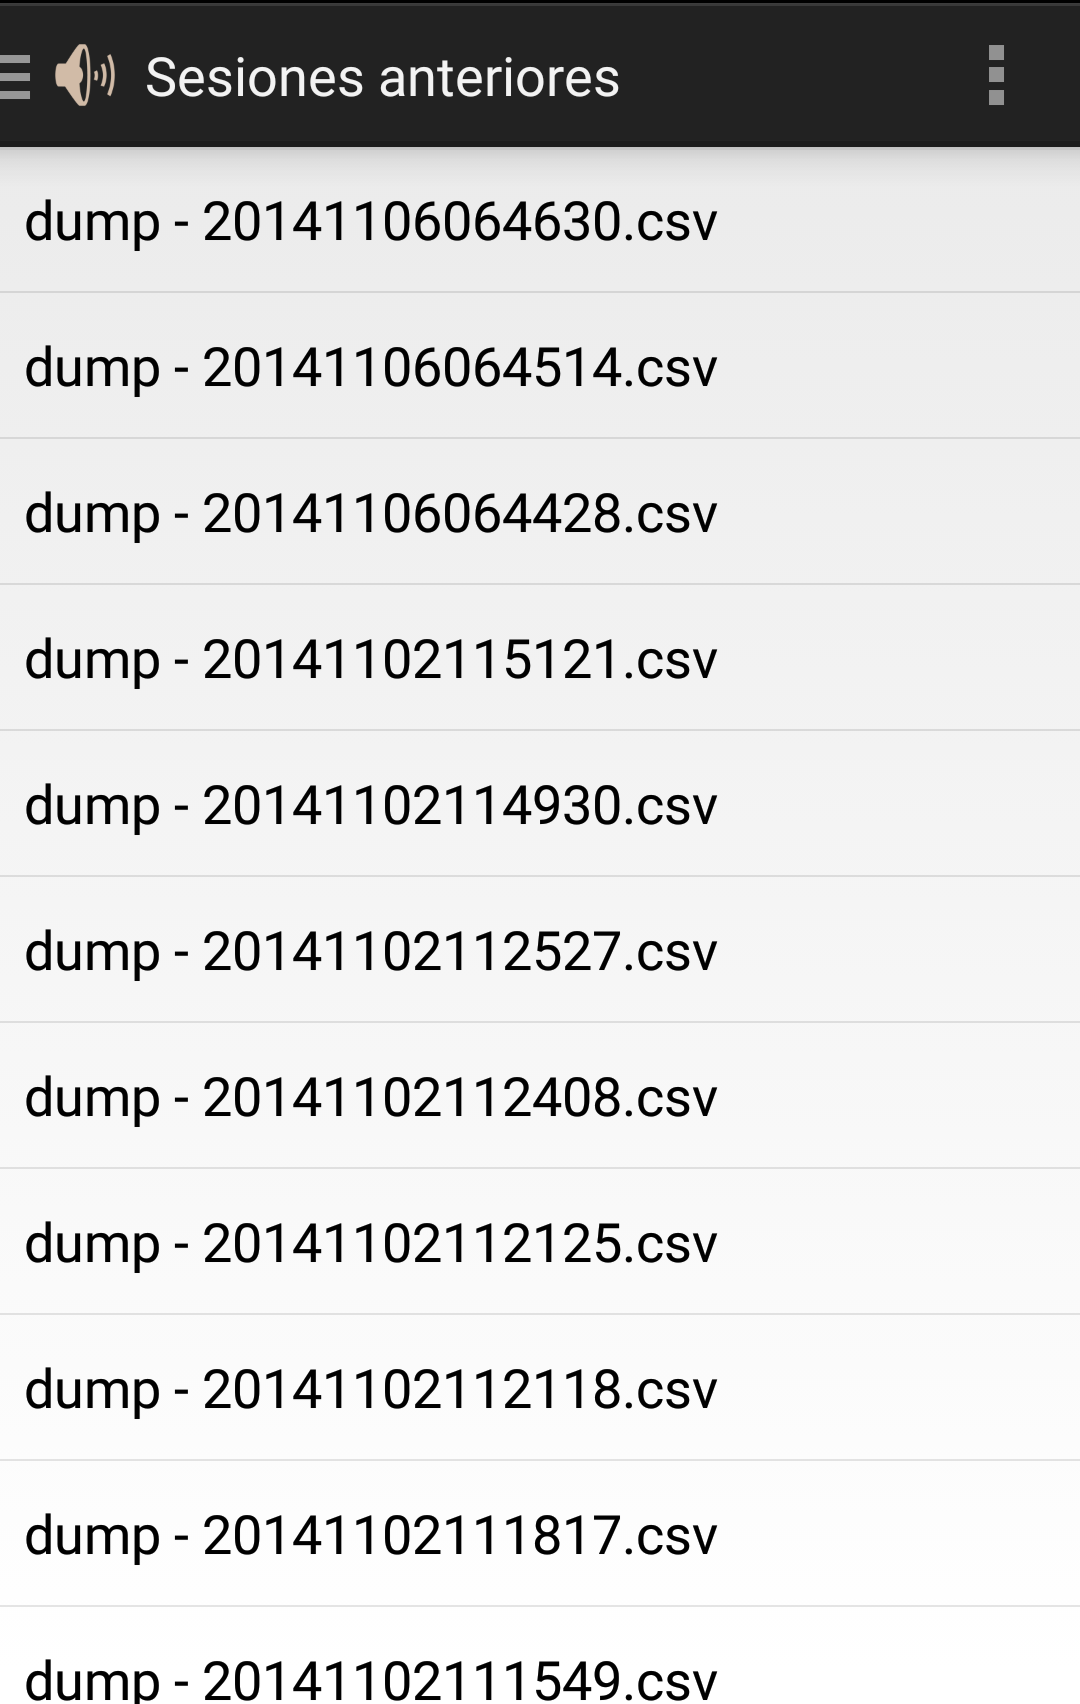
\includegraphics[height=11cm]{graphs/sessions.png} \caption{Fragmento \ttw{Sesiones} mostrando la lista de archivos de sesiones anteriores.}\label{fig:screen:sessions}%
 \end{minipage}
 \hfill
\begin{minipage}{0.45\textwidth}\centering%
 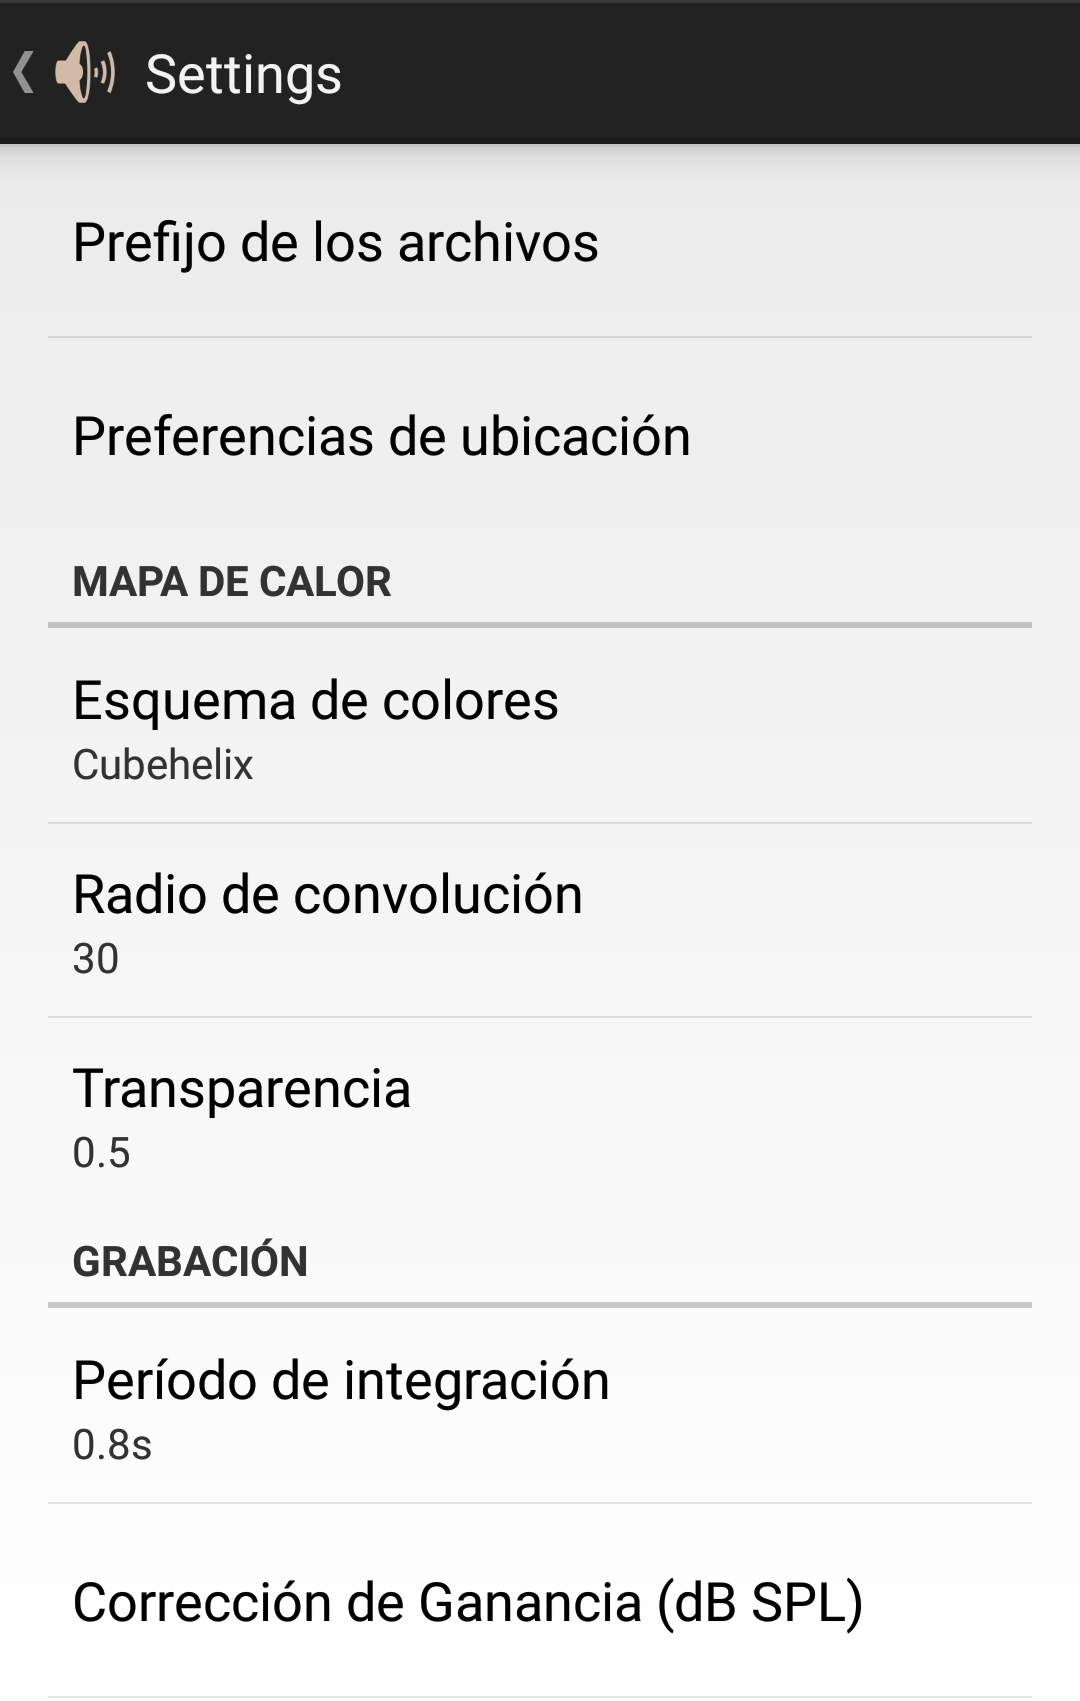
\includegraphics[height=11cm]{graphs/settings.png} \caption{Actividad \ttw{Opciones}, donde se configuran distintos aspectos de la aplicación.}\label{fig:screen:settings}
\end{minipage}
\end{figure}

    Una vez ejecutada la aplicación, se inicia la actividad del cajón de navegación, mostrando el fragmento \ttw{Mapa de Calor}. El mapa está centrado en la ubicación actual, tal y como muestra la figura \ref{fig:screen:location}. Esta permite utilizar el mapa de manera idéntica a la que lo haríamos en la aplicación Google Maps. Desde esta pantalla, se puede o bien \ttw{Cargar datos} de alguna sesión de grabación o abrir el cajón de navegación, ya sea pulsando sobre el icono de la aplicación, o haciendo el gesto característico de este patrón de diseño de interfaz de usuario, que es arrastrar desde fuera del borde izquierdo hacia dentro.
    
    Una vez abierto el cajón de navegación, se presentan los distintos elementos del menú. Apreciable en la figura \ref{fig:screen:navdrawer}, el cajón de navegación da acceso a los fragmentos \ttw{Mapa de calor}, \ttw{Medición}, \ttw{Sesiones anteriores} y a la actividad de \ttw{Opciones}.
    
    Para realizar una nueva medición, se hace click en el elemento \ttw{Medición} del cajón de navegación, para hacer aparecer al fragmento \ttw{Medición} en pantalla. Al pulsar el botón que lee \ttw{Empezar medición}, el proceso de medición comienza. Los servicios en segundo plano son iniciados, y tras un breve retardo empiezan a aparecer en pantalla valores de la medición. 
    
    Conforme los valores van siendo medidos y calculados, el histórico de las últimas muestras se dibuja en pantalla en el área dispuesta a tal efecto. Durante todo el proceso, los datos recabados son grabados a la memoria del dispositivo en segundo plano.
    
    Una vez finalizada la medida, se presiona el botón \ttw{Parar medición}, y los servicios en segundo plano de la aplicación vuelven al reposo. Abriendo de nuevo el cajón de navegación, es posible acceder al fragmento de \ttw{Sesiones anteriores}, donde se muestra una lista de todos los archivos producidos en grabaciones anteriores. De la misma manera, es posible volver al fragmento \ttw{Mapa de calor}.
    
    De vuelta en el fragmento \ttw{Mapa de calor}, al pulsar el botón \ttw{Cargar datos}, se mostrará un diálogo con la lista de todos los archivos producidos en grabaciones anteriores. Al seleccionar uno de estos archivos, la aplicación calcula el mapa de calor resultante de los datos contenidos en dicho archivo, y lo superpone al mapa actual. En la figura \ref{fig:screen:heatmap} se aprecia un ejemplo de dicho comportamiento. Cambiando el nivel de acercamiento del mapa, se obtienen distintos niveles de agregamiento de los datos.
    
    La aplicación dispone también de una actividad de \ttw{Opciones}, donde se pueden configurar varios aspectos del comportamiento de la misma. El acceso a dicha actividad, puede ser llevado a cabo de dos maneras. La primera es usando el mismo cajón de navegación que para acceder al resto de los fragmentos de la aplicación. La segunda es haciendo uso del menú contextual que aparece al tocar en la barra de acción cuando nos encontramos en cualquier fragmento que no sea \ttw{Mapa de calor}, ya que en este último el botón \ttw{Cargar datos} ocupa su lugar. En la figura \ref{fig:screen:settings} se observa el contenido de dicha actividad.
    
    Dentro de la actividad \ttw{Opciones}, cabe la posibilidad de realizar múltiples configuraciones. Estas son:
    
    \begin{itemize}
    \item Renombrar el prefijo utilizado en el nombre de los archivos de guardado en el almacenamiento del dispositivo
    \item Acceder a las preferencias de ubicación del sistema, para poder habilitar cómodamente la medida de alta precisión
    \item Cambiar el esquema de colores utilizado en la generación del mapa de calor
    \item Alterar el radio de convolución que se utiliza en la generación del mapa de calor
    \item Modificar la transparencia con la que el mapa de calor se superpone al mapa geográfico
    \item Variar el período de integración con el que se realizan las medidas
    \item Aplicar una corrección de ganancia a las medidas
    \end{itemize}
    
    Por último, cabe destacar que, al guardarse los archivos en la memoria del dispositivo, estos pueden ser extraídos y utilizados posteriormente, ya sea para ser procesados, representados de diferente manera o agregados con otros datos. Depende del modelo de teléfono inteligente utilizado, este dispondrá o no de tarjeta de almacenamiento externa. La aplicación preferirá guardar sus datos en la tarjeta de almacenamiento externa, y solo cuando esta no exista, se grabarán los datos en la memoria interna del teléfono. Un ejemplo del contenido de un archivo de sesión de captura de la aplicación está disponible en la figura \ref{fig:dump:file}.
    
\begin{figure}[h] \centering
\begin{boxedverbatim}
"magnitude","latitude","longitude","accuracy","timestamp"
"62.09779","51.1157184","17.0541213","12.618","31/01/2015 04:13:03"
"60.62046","51.1157184","17.0541213","12.618","31/01/2015 04:13:03"
"57.23939","51.1157184","17.0541213","12.618","31/01/2015 04:13:03"
"55.49906","51.1157184","17.0541213","12.618","31/01/2015 04:13:03"
"56.60217","51.1157184","17.0541213","12.618","31/01/2015 04:13:03"
"63.38877","51.1157184","17.0541213","12.618","31/01/2015 04:13:03"
"64.22864","51.1157184","17.0541213","12.618","31/01/2015 04:13:03"
"72.13268","51.1157184","17.0541213","12.618","31/01/2015 04:13:03"
"78.58884","51.1157184","17.0541213","12.618","31/01/2015 04:13:03"
\end{boxedverbatim}
\caption{Extracto de un archivo CSV producido por la aplicación}
\label{fig:dump:file}
\end{figure}

\section{Precisión de las medidas}
    Para cerciorarse de que los valores de nivel de presión sonora mostrados en la aplicación se ajustan a la realidad, es necesario comparar los valores para una misma fuente con los obtenidos por un aparato de medición calibrado.

    Tras realizar dichas medidas, la aplicación deberá de ser configurada conforme a los resultados obtenidos, introduciendo los parámetros pertinentes en la pantalla dispuesta a dicho efecto.

    Dicho proceso es necesario para cada micrófono distinto que sea usado con la aplicación, ya sea por usarla en un teléfono distinto o por utilizar un micrófono externo, ya que las características de cada uno varían, y no puede garantizarse la fidelidad de los resultados de un micrófono con los parámetros de otro.
    
\subsection{Realización de medidas en laboratorio}
    Para las pruebas de calibrado del nivel de presión sonora, se han realizado en el laboratorio medidas de nivel de presión sonora emitido por un monitor de estudio, primero por un sonómetro calibrado, y después por la aplicación.

    El sonómetro utilizado ha sido el Svantek SVAN 977.

    El micrófono utilizado por la aplicación ha sido el integrado en el teléfono, modelo LG Nexus 5. Según \cite{n5-svcman}, es un micrófono del tipo microelectromecánico, o MEMS según sus siglas en inglés, de la marca Goertek. Sin embargo, la hoja de características del micrófono no está disponible.

    Los resultados de la batería de pruebas pueden observarse en la tabla \ref{tab:SAR}. Es notoria la similitud de las mediciones para el tono puro, y un resultado del todo esperado dado que cae dentro del rango de frecuencias típicas de trabajo de un micrófono de un dispositivo móvil.
    
\begin{table}[h]%
\centering
\begin{tabular}{|l|c|c|}
    \hline
    \hline
    \tbf{Aparato}&\tbf{Sonómetro} &\tbf{Nexus 5}\\ \hline 
    \tbf{Tono 440 Hz} &68.7 dB& 68.6 dB \\ \hline
    \tbf{Fuente sonora apagada}& 37.4 dB& 43.2 dB \\ \hline
    \tbf{Ruido blanco} &  69.3 dB & 62.6 dB\\ \hline
    \tbf{Ruido Rosa} & 69.2 dB& 64.1 dB \\ \hline
    \tbf{Canción}& 63.1 dB & 59.3 dB\\ \hline
    \hline 
\end{tabular}
\caption{Tabla de comparacion de mediciones} \label{tab:SAR}
\end{table}

    Sin embargo, cuanto más nos alejamos de dicho funcionamiento típico del micrófono del dispositivo móvil, es posible observar mayores discrepancias. En el límite inferior, se observa cómo la sensibilidad de dicho tipo de micrófonos es limitada, y no es capaz de detectar niveles menores de alrededor de 43 dB.

    Presentado ante un ruido blanco, la aplicación reporta un nivel menor que el observado en la lectura del sonómetro. Es de suponer que esto es debido al sonómetro siendo capaz de abarcar un espectro mayor de frecuencias en su medición, y por tanto recibiendo unas lecturas más altas. 

\subsection{Realización de medidas de campo}
\subsubsection{Calle concurrida}
\begin{figure}[H] \centering
 \begin{minipage}{0.45\textwidth}\centering
    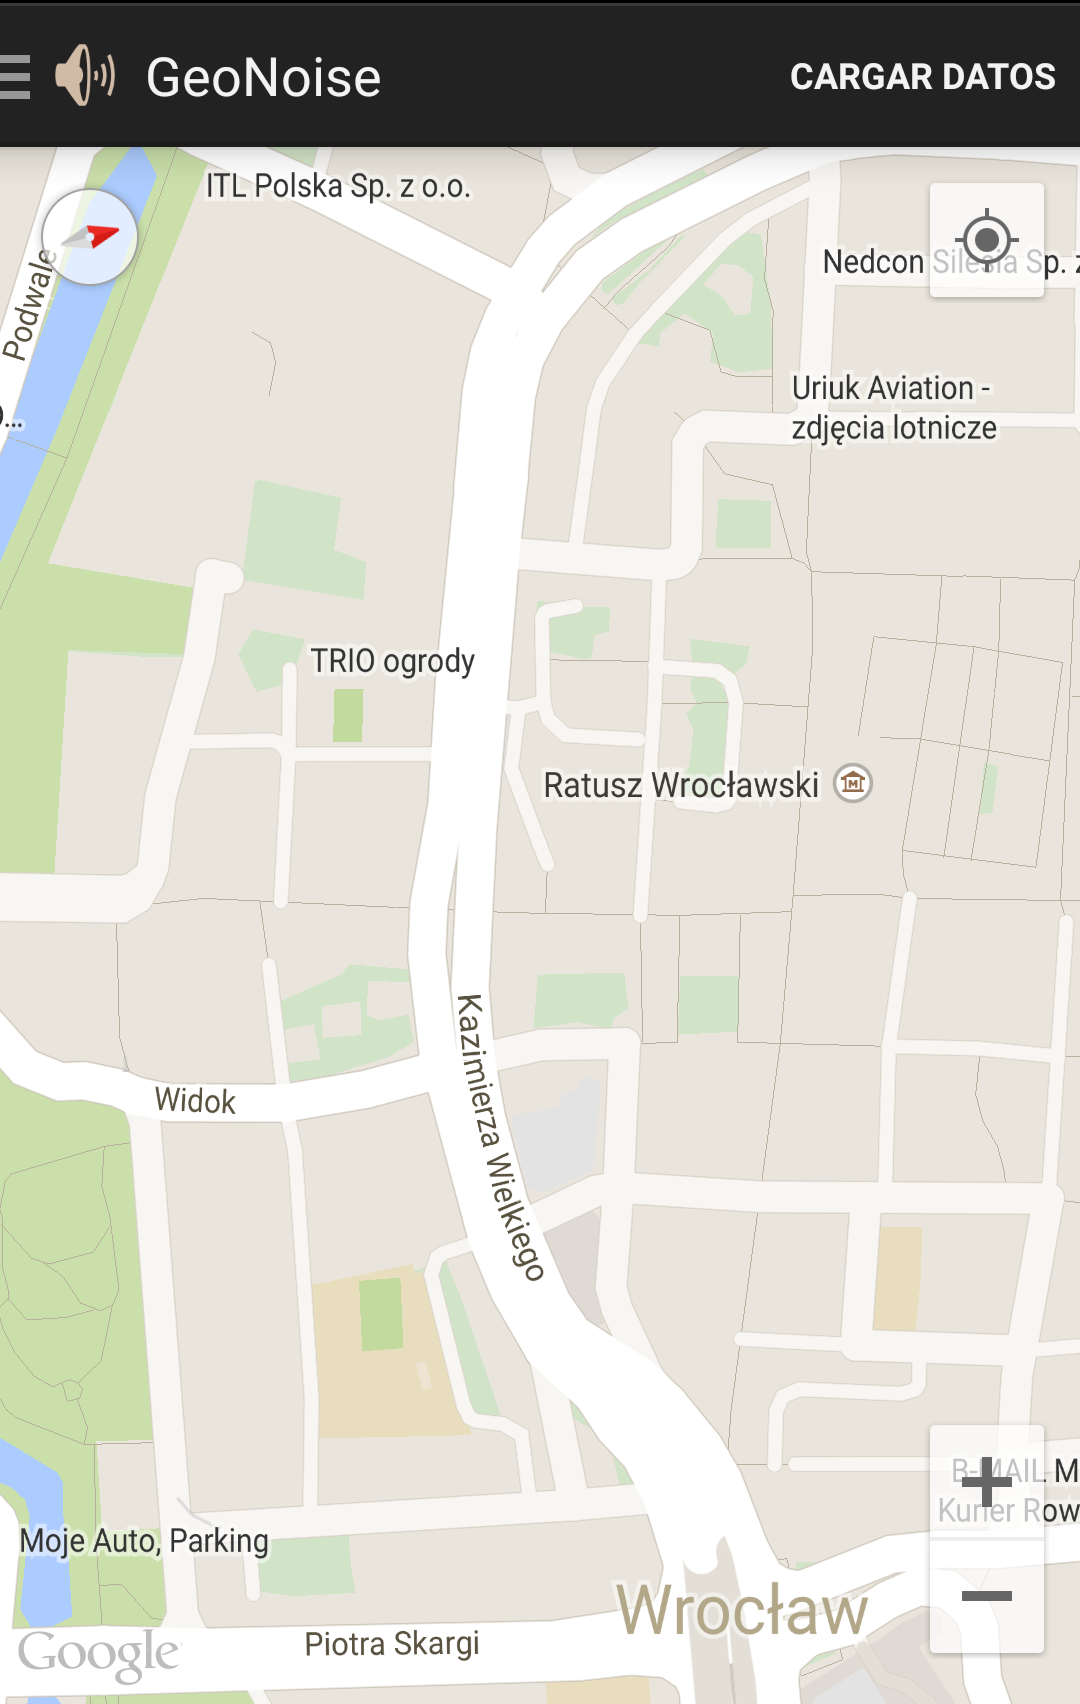
\includegraphics[height=11cm]{graphs/road.png} \caption{Vista del mapa de la calle antes de superponer la medida.}\label{fig:screen:road}
 \end{minipage}
 \hfill
\begin{minipage}{0.45\textwidth}\centering
    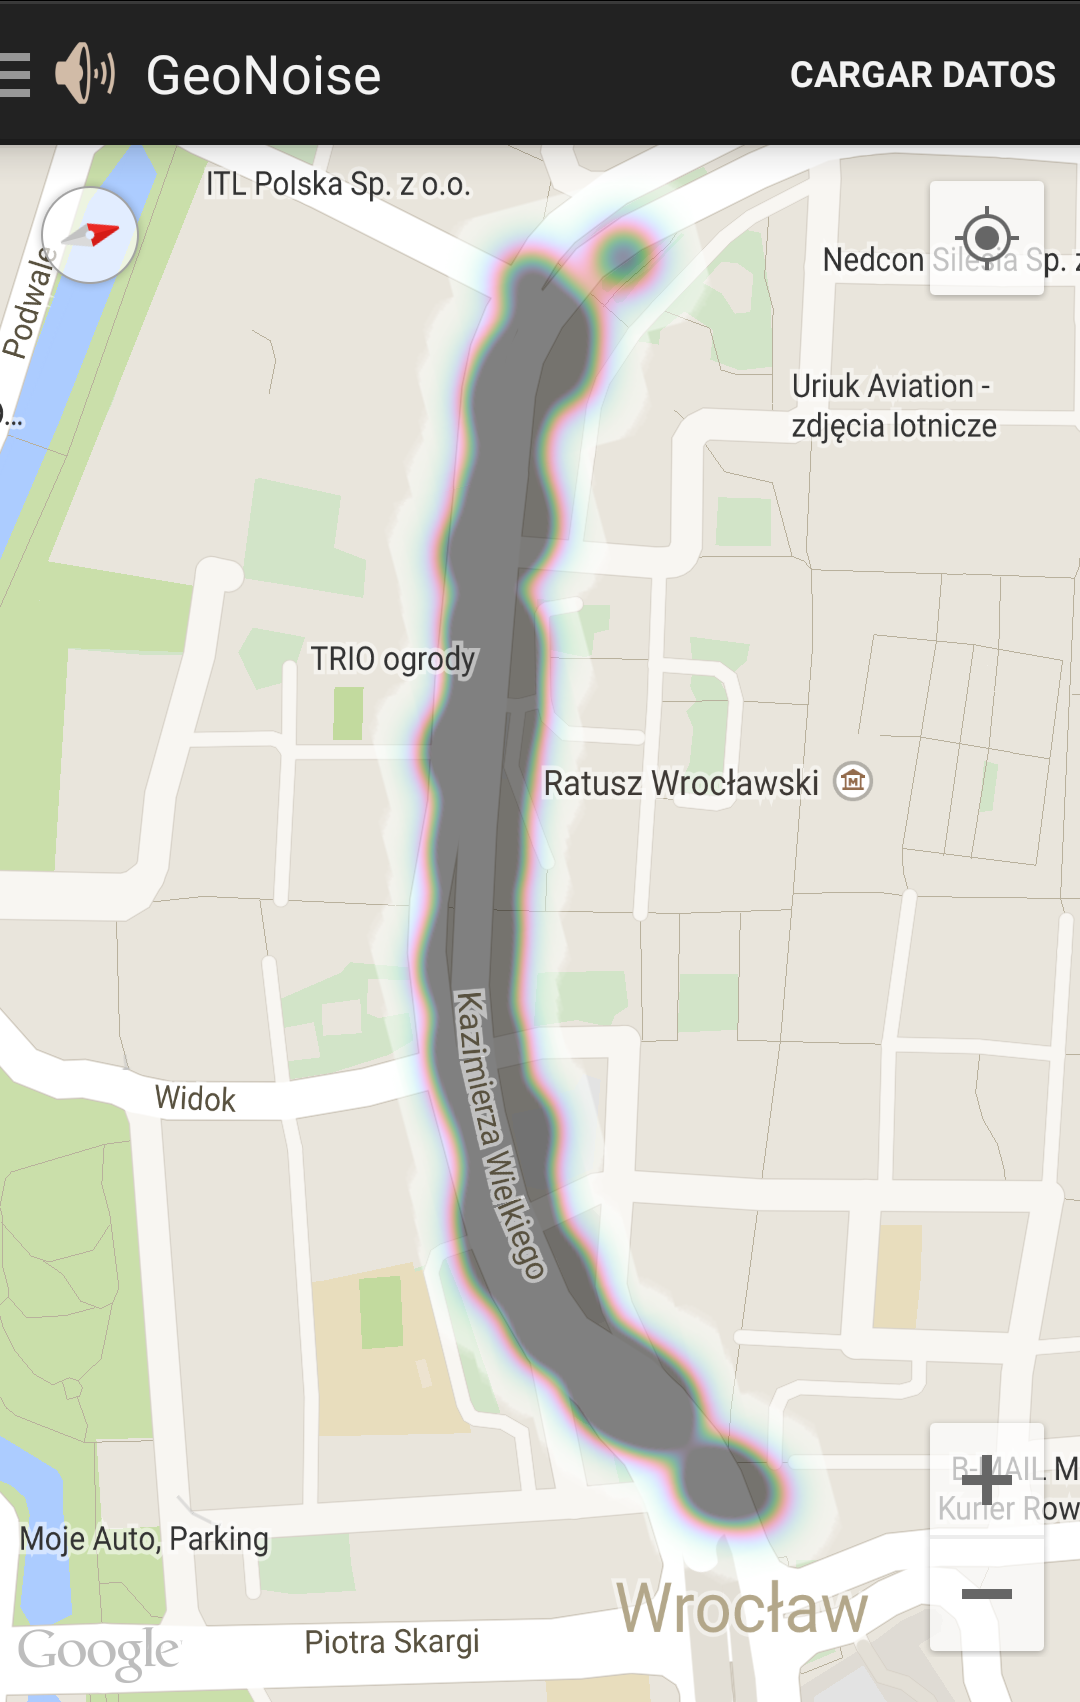
\includegraphics[height=11cm]{graphs/roadmapped.png} \caption{Vista del mapa de la calle con la medida superpuesta.}\label{fig:screen:roadmapped}
\end{minipage}
\end{figure}
    Para el escenario de calle concurrida, se ha elegido la calle Kazimierza Wielkiego de Wrocław, una de las calles principales de la ciudad, vertical en la figura  \ref{fig:screen:road}. Se trata de una calle concurrida, con un volumen de tráfico cosiderable, y por tanto es de esperar un nivel de ruido elevado. Tras la realización de las medidas, es posible observar en la figura \ref{fig:screen:roadmapped} cómo prácticamente la totalidad del terreno cubierto en la medida se encuentra en el valor más alto.

\subsubsection{Parque tranquilo}
\begin{figure}[H] \centering
 \begin{minipage}{0.45\textwidth}\centering
    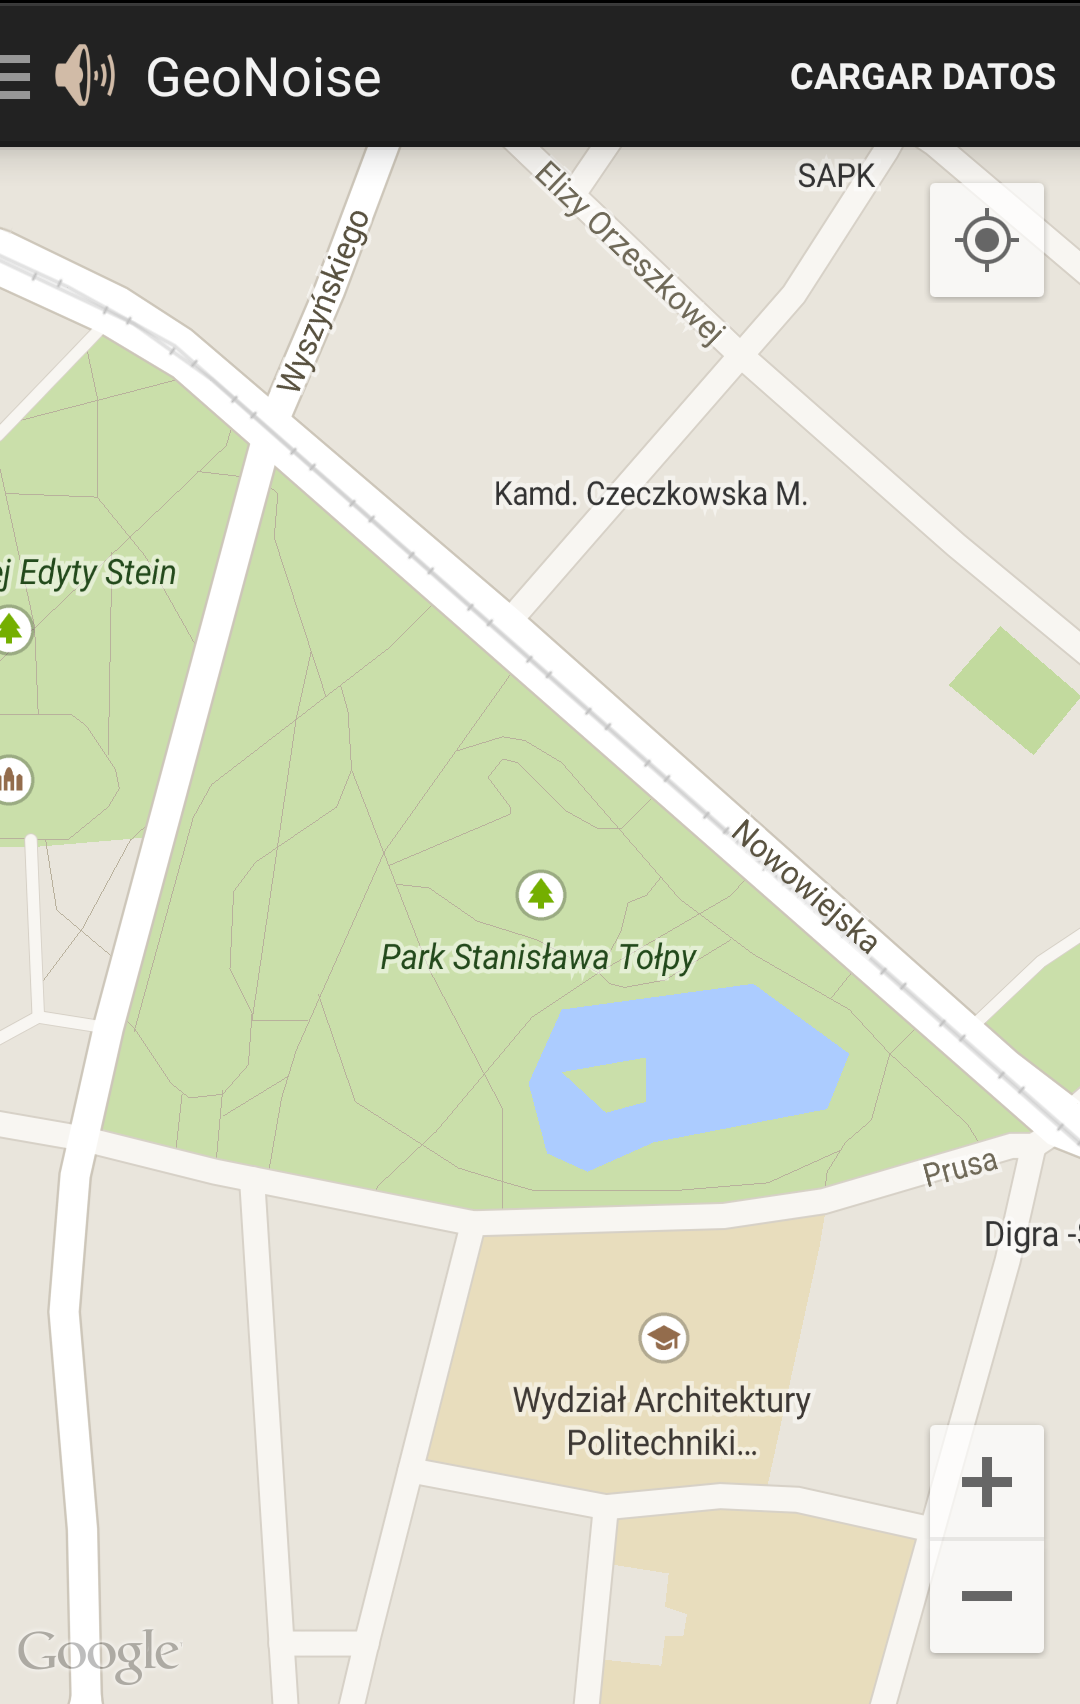
\includegraphics[height=11cm]{graphs/park.png} \caption{Vista del mapa del parque antes de superponer la medida.}\label{fig:screen:park}
 \end{minipage}
 \hfill
\begin{minipage}{0.45\textwidth}\centering
    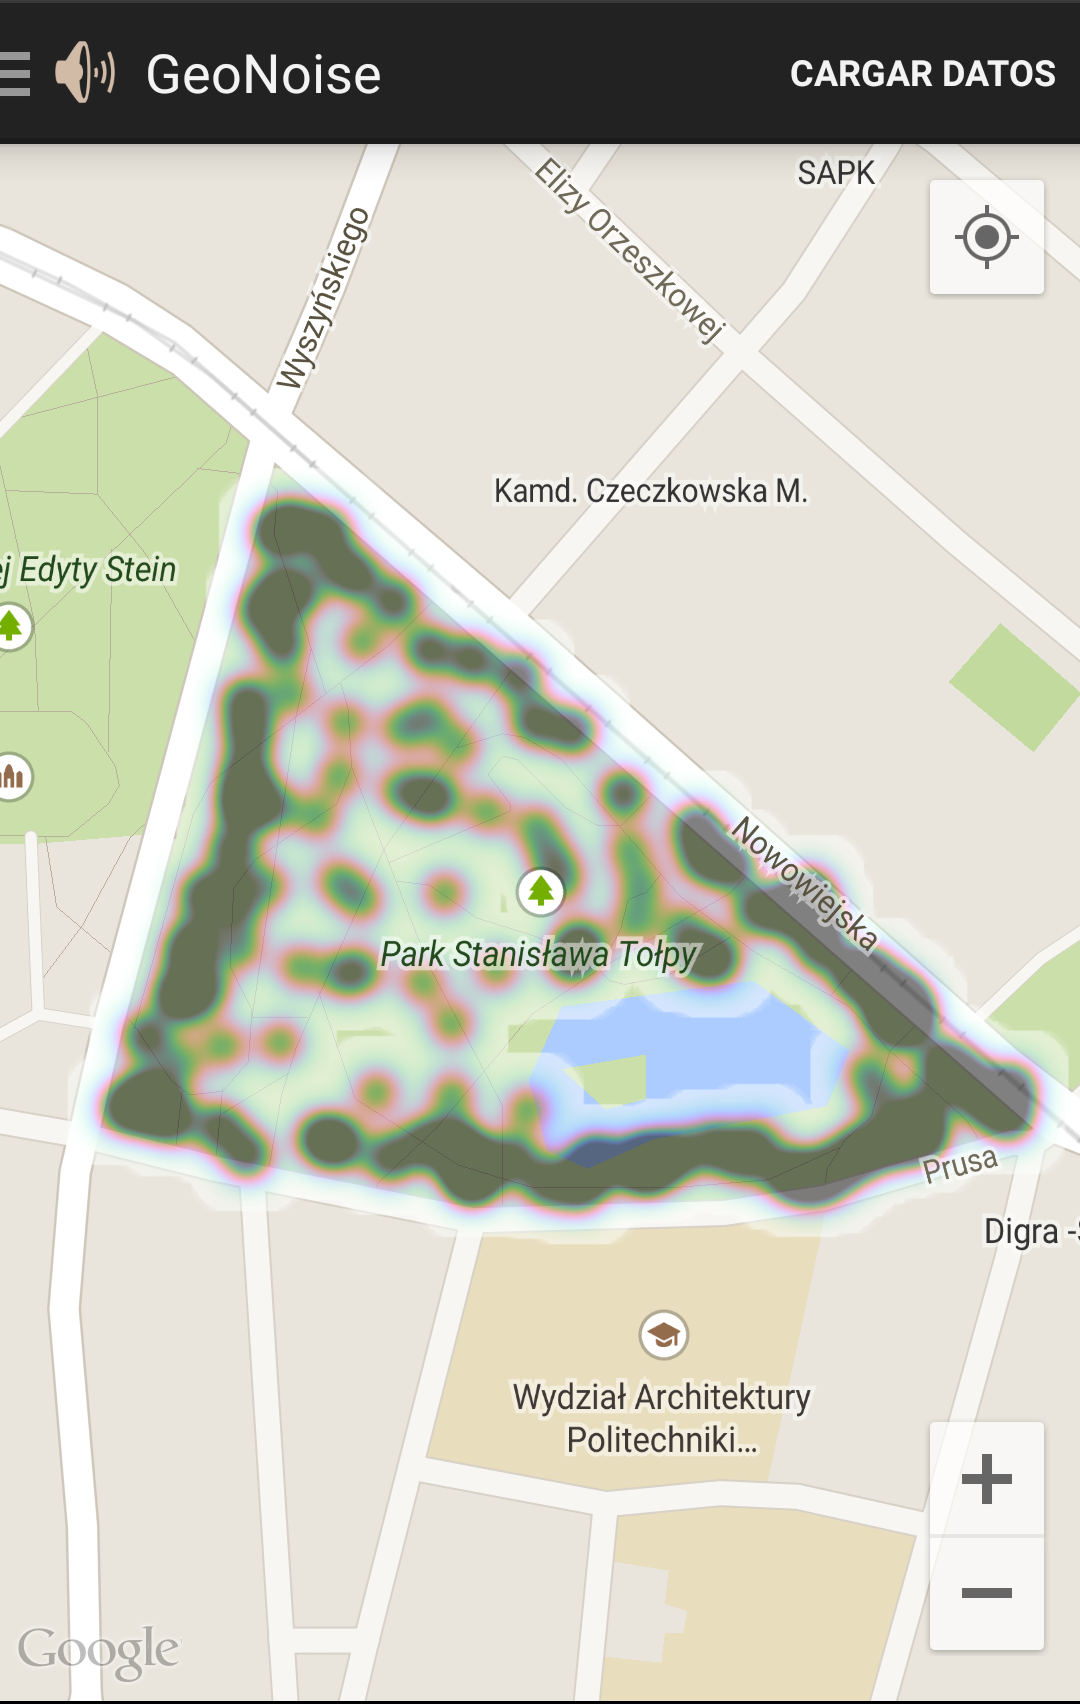
\includegraphics[height=11cm]{graphs/parkmapped.png} \caption{Vista del mapa del tranquilo con la medida superpuesta.}\label{fig:screen:parkmapped}
\end{minipage}
\end{figure}
    Para el escenario de parque tranquilo, se ha elegido el parque Stanisława Tołpy de Wrocław, un parque de tamaño mediano con abundante vegetación, cuya disposición se observa en la figura \ref{fig:screen:park}. En este caso, se da una mayor diversidad de medidas. Las medidas de mayor intensidad se encuentran cerca de la carretera, y disminuyen de intensidad conforme se aproxima al centro del parque.


\section{Realización de los objectivos}

\subsection{Capacidad de medir la magnitud del ruido ambiente}
La aplicación es capaz de medir la magnitud de ruido ambiente en cualquier momento dado, tan solo hay que comenzar la captación y se muestra un valor estimado en decibelios. Podemos observar que dicho objetivo se cumple en la figura \ref{fig:screen:measure}.

\subsection{Capacidad de determinar la posición del dispositivo}
La aplicación cumple con el objetivo de ser capaz de determinar la posición absoluta del dispositivo móvil, ya sea dentro del mapa utilizado para representar los datos obtenidos previamente, o durante la operación de recabado de datos. Es posible apreciar cómo el punto azul determina nuestra posición actual en la figura \ref{fig:screen:location}. Durante la medición no se muestra de forma directa la posición absoluta medida, pero es tenida en cuenta en todo momento de la misma.


\subsection{Capacidad de asociar ambas mediciones}
La aplicación vincula en cada operación de muestreo la magnitud medida y la posición absoluta medida, de manera que sea posible conocer a qué punto geográfico pertenece cada medida. Es posible observar dicha asociación en el contenido del archivo creado por cada sesión de grabación, como puede observarse en la figura \ref{fig:dump:file}.

\subsection{Capacidad de almacenar los datos obtenidos}
Los datos son almacenados inmediatamente después de la finalización de la sesión de grabado a la memoria del dispositivo. Estos pueden ser recuperados conectando el dispositivo móvil a un ordenador personal, o bien representados dentro de la propia aplicación. Una muestra del contenido de un archivo de almacenamiento se puede observar en la figura \ref{fig:dump:file}.

\subsection{Capacidad de mostrar los datos obtenidos sobre un mapa}
Una vez finalizada una sesión de grabación, la aplicación está capacitada para mostrar un listado de las sesiones finalizadas. Una vez seleccionada la sesión que se quiere representar sobre el mapa, la pantalla se actualiza mostrando los datos pertinentes, tal y como se aprecia en la figura \ref{fig:screen:heatmap}.

\chapterend{}